%!TEX root = ../dokumentation.tex

%TODO: Einleitung überarbeiten
\chapter{Implementierung}\label{cha:Implementierung}
\section{Datenbank, Login und Registrierung}\label{Datenbank}
Zu Beginn verbindet sich der Server mit der Datenbank. Server und Datenbank können über einen definierten Port kommunizieren. Der Server kann mittels Datenbankabfragen auf die Daten zugreifen. Wenn sich ein neuer User registriert, sendet der Client dem Server den Usernamen und das Passwort. Der Server fordert nun von der Datenbank gespeicherte Daten an, die den Usernamen und das Passwort enthalten. Wenn die Antwort der Datenbank ein leeres Objekt ist, ist noch kein User mit dem Usernamen und dem Passwort registriert und in der Datenbank wird ein neuer Eintrag erstellt. 

Folgendes Bild zeigt den Ablauf des Logins:
\begin{figure}[H]
\centering
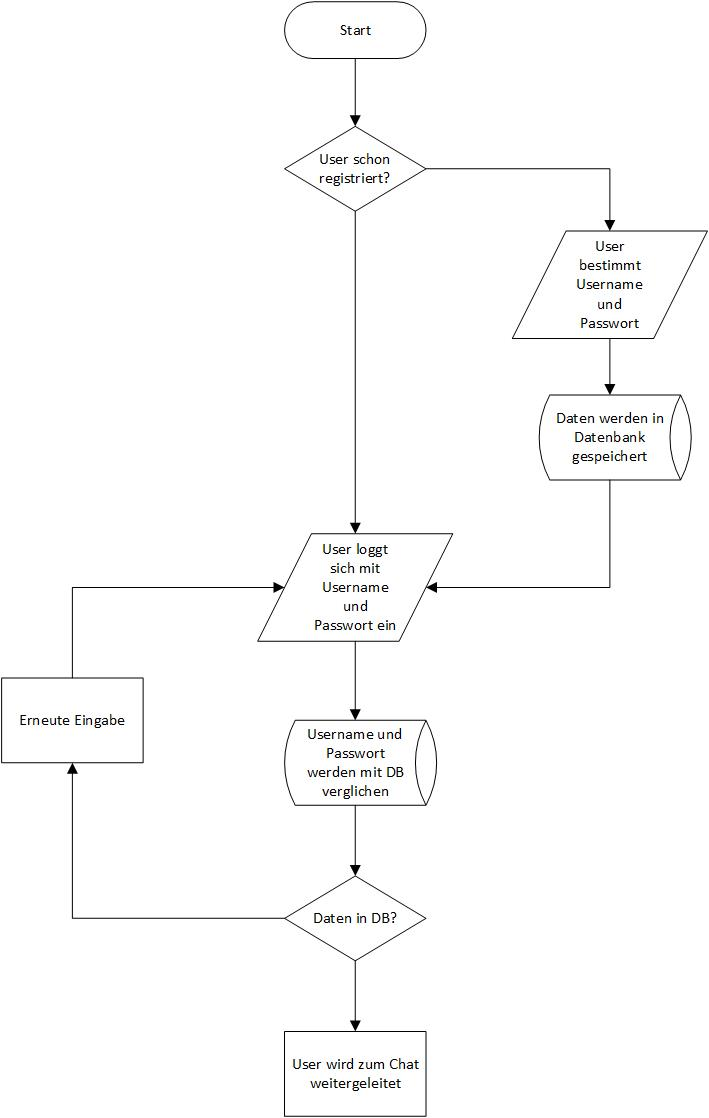
\includegraphics[width=0.5\textwidth]{images/login.jpg}
\caption{Flussdiagramm des Loginprozesses}
\end{figure}

Im folgenden ist der Verbindungsaufbau mit der MongoDB gezeigt. In der URL ist die Portnummer des MongoDB-Container, über den die Verbindung aufgebaut wird. Der darauffolgende Name ist der Name des Docker-Containers, aus dem die Datenbank aufgerufen wird.
In der letzten Zeile wird das auf definierte Datenbankschema verwiesen. 

\begin{lstlisting}[language=bash, caption={Verbindungsaufbau mit der MongoDB}, label=lis:POST]

mongoose
  .connect(
    'mongodb://mongo:27017/docker-node-mongo',
    { useNewUrlParser: true }
  )
  .then(() => console.log('MongoDB Connected'))
  .catch(err => console.log(err));

const User = require('./js/user');

\end{lstlisting}

In folgendem Schema ist definiert, was für Attribute das in der Datenbank gespeicherte Objekt besitzt. 

\begin{lstlisting}[language=bash, caption={Datenschema in der MongoDB}, label=lis:POST]

const mongoose = require('mongoose');
const Schema = mongoose.Schema;

const UserSchema = new Schema({
  name: {
    type: String,
    required: true
  },
  password: {
    type: String,
    required:true
  }
});

module.exports = User = mongoose.model('User', UserSchema);

\end{lstlisting}

\section{Spiellogik}\label{sec:Spiellogik}
Der User kann das Spiel über einen Knopf starten. Nun muss er warten bis ein anderer User das Spiel ebenfalls startet. Nachdem das Spiel gestartet ist, kann der User, der momentan an der Reihe anhand von Knöpfen über halb des Spielfeldes wählen, in welche Reihe er setzen möchte. Falls das Setzen nicht möglich ist, da die Reihe voll ist, darf er erneut setzen. Wenn ein Spieler einen Stein setzen möchte, obwohl er nicht an der Reihe ist, wird dieser nicht gesetzt. Nach jedem Zug wird geprüft, ob das Spiel endet. Wenn ja, kann ein neues Spiel begonnen werden.

\begin{figure}[H]
\centering
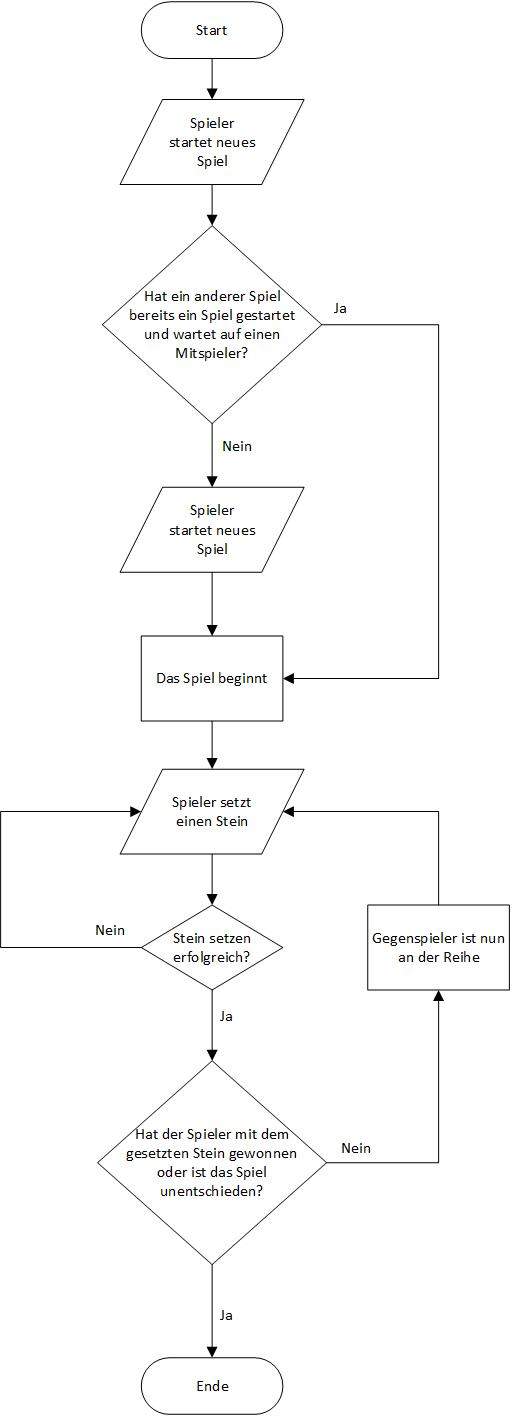
\includegraphics[width=0.5\textwidth]{images/spiellogik.jpg}
\caption{Flussdiagramm des Spielablaufs}
\end{figure}

\section{Erkennung des Spielendes}\label{sec:GameOver}
Es gibt zwei Szenarien, unter denen das Spiel zu Ende ist. Entweder gewinnt ein Spieler oder das Spiel endet unentschieden. Unentschieden ist das Spiel, wenn das Spielfeld komplett gefüllt ist, aber kein Spieler eine Reihe aus vier Steinen aufbauen konnte.
Bei einem Gewinn sind drei verschiedene Szenarien zu unterscheiden. Eine Reihe aus vier Spielsteinen des gleichen Spielers kann horizontal, vertikal oder diagonal auftreten. Wenn die Reihe diagonal gebildet wird, kann noch zwischen von links unten nach rechts oben und von rechts unten nach links oben unterschieden werden. Alle diese Fälle müssen geprüft werden.

\section{Docker Compose}\label{sec:Docker Compose}
Im Docker-Compose-File sind die zu verwaltenen Container aufgezählt mitsamt der Portnummern, über den auf die Container zugegriffen werden kann.

In der ersten Zeile wird das Docker Compose File Format genannt. Version 3 ist die aktuelle Version. In den folgenden Zeilen werden die einzelnen Services, also die einzelnen Docker-Container festgelegt.
Die Portnummern beschreiben das Abbild von interne auf externe Portnummer. Mit Hilfe der externen Portnummer auf der rechten Seite können die Docker-Container miteinander kommunizieren.
In Zeile 6 wird der Pfad hinterlegt, in dem das Docker-File hinterlegt ist, welches die build-Funktion spezifiert. 
In Zeile 16 ist der Name des erstellten Images festgelegt, aus dem der Container gestartet wird. Der Container-Name in Zeile 4 beschreibt den Namen des Docker-Containers, anstatt einen default Namen zu benutzen. Links in Zeile 10 benennt Links zu anderen Containern außerhalb des Docker-Compose-Files. Referenz: https://docs.docker.com/compose/compose-file/
\begin{lstlisting}[language=bash, caption={docker-compose.yml-File}, label=lis:POST]
version: '3'
services:
  app:
    container_name: docker-node-mongo
    restart: always
    build: .
    ports:
      - '80:3000'
      - '8181:8181'
    links:
      - mongo
  mongo:
    container_name: mongo
    image: mongo
    ports:
      - '27017:27017'


\end{lstlisting}


